\documentclass[pdflatex,sn-mathphys-num]{sn-jnl}

\usepackage{graphicx}
\usepackage{multirow}
\usepackage{amsmath,amssymb,amsfonts}
\usepackage{amsthm}
\usepackage{mathrsfs}
\usepackage[title]{appendix}
\usepackage{xcolor}
\usepackage{textcomp}
\usepackage{manyfoot}
\usepackage{booktabs}
\usepackage{algorithm}
\usepackage{algorithmicx}
\usepackage{algpseudocode}
\usepackage{listings}
\usepackage{tabularx}
\usepackage{array}
\usepackage{longtable}
\usepackage{colortbl}

\raggedbottom

\begin{document}

\title[Cloud-Native Software Localization Pipelines]{Benchmarking Neural Machine Translation for Cloud-Native Software Localization Pipelines: A Multi-Metric Evaluation Across High-Resource and Low-Resource Languages}

\author*[1]{\fnm{Neeraj Kumar} \sur{Sharma}}\email{p20220505@hyderabad.bits-pilani.ac.in}
\author[1]{\fnm{Subhrakanta} \sur{Panda}}\email{spanda@hyderabad.bits-pilani.ac.in}
\author[1]{\fnm{Lalita Bhanu Murthy} \sur{Neti}}\email{bhanu@hyderabad.bits-pilani.ac.in}

\affil*[1]{\orgname{BITS Pilani, Hyderabad Campus}, \city{Hyderabad}, \postcode{500078}, \country{India}}

\abstract{As artificial intelligence and cloud-native architectures become integral to modern software delivery, the demand for automated, scalable multilingual localization across distributed cloud platforms grows rapidly. Modern cloud services, serverless CI/CD pipelines, and IoT ecosystems depend on short, context-dependent user interface (UI) strings containing technical artifacts such as keyboard accelerators, variable placeholders, and accessibility labels. Ensuring translation fidelity without breaking automated deployment velocity requires rigorous, intelligent model selection within cloud translation microservices. This paper benchmarks four alternative neural machine translation (NMT) systems (one commercial, Microsoft Translator, and three open-source: NLLB-200, MADLAD-400, and IndicTrans2) against Google Translate as the industry-standard baseline across twelve language pairs spanning high-resource and low-resource (Indic) languages. Using a fixed test set of 10,228 authentic software UI strings drawn from the KDE desktop environment, we employ a multi-metric assessment framework comprising BLEU, METEOR, chrF++, ROUGE-L, TER, COMET, and BERTScore, supplemented by CometKiwi reference-free quality estimation for independent pipeline validation. Results demonstrate that open-source models (NLLB-200, IndicTrans2) deliver competitive performance for low-resource Indic languages, while commercial systems maintain superiority for high-resource European pairs. These findings provide data-driven, AI-informed routing recommendations for embedding intelligent translation backends into cloud-native localization architectures and serverless delivery workflows.}

\keywords{Cloud Computing, Cloud-Native Localization, Neural Machine Translation, CI/CD Pipelines, Serverless Architectures, Multilingual Software Delivery, Benchmarking}

\maketitle

\section{Introduction}

\subsection{Background and Motivation in Cloud Ecosystems}

The convergence of cloud computing, pervasive IoT ecosystems, and artificial intelligence has produced a new generation of ubiquitous assistive technologies~\cite{1,2,3,4}. These platforms rely heavily on accurately localized multilingual interfaces to deliver accessible, human-centered services across distributed deployments.

Within modern cloud-native architectures, continuous integration and continuous delivery (CI/CD) pipelines automate the build, test, and release lifecycle, reducing release cycles from months to hours~\cite{5,6}. However, while core software engineering has achieved high velocity through cloud automation, software localization (the adaptation of applications to the linguistic, cultural, and regulatory expectations of target markets) has historically lagged behind, often treated as a manual post-development bottleneck. 

To bridge this gap, recent advancements have introduced cloud-native and serverless frameworks for continuous software localization~\cite{7}. As detailed in cloud localization delivery models, automated translation microservices must operate elastically within cloud storage and event-driven orchestration layers. Yet, embedding neural machine translation (NMT)~\cite{8} into automated cloud pipelines introduces distinct technical hurdles: UI strings in cloud platforms, IoT dashboards, and distributed applications are characteristically short (often 1 to 3 words), highly context-dependent, and interspersed with technical artifacts such as keyboard accelerators (e.g., \texttt{\&Delete item}), variable placeholders (e.g., \texttt{Save as \%1}), and concatenated identifiers~\cite{9,10}. Translation errors in these elements can corrupt cloud interfaces, break runtime parsing, or compromise accessibility for assistive technology users.

Google Translate has become the de facto baseline for cloud-based translation services, serving massive request volumes across global infrastructure. For cloud architects and developers building multi-region platforms, evaluating how alternative commercial and open-source NMT systems perform relative to this baseline, particularly across diverse language pairs including underserved Indic languages, is critical for optimizing intelligent translation microservices and serverless routing layers.

\subsection{Research Gap and Contributions}

While existing literature has examined individual NMT systems and evaluation metrics, there remains a gap in comprehensive, AI-driven multi-system benchmarking specifically targeting the short, artifact-laden interface strings characteristic of assistive technologies, IoT devices, and pervasive computing systems across both high-resource and low-resource language pairs. Furthermore, most evaluation studies rely exclusively on reference-based metrics, without independent validation through reference-free quality estimation, and few address the accessibility and ubiquitous deployment implications of translation quality for underserved language communities.

This paper makes the following contributions:

\begin{enumerate}
\item We establish an AI-driven benchmarking framework that uses Google Translate as the industry-standard baseline against which four alternative NMT systems (three general-purpose, one Indic-specialized) are systematically compared for the interface strings typical of assistive technologies, IoT systems, and pervasive computing environments.
\item We conduct a comprehensive evaluation across twelve language pairs (five high-resource, seven low-resource including six Indic languages) using seven evaluation metrics and a corpus of authentic open-source software UI strings.
\item We employ CometKiwi, a reference-free quality estimation metric, to independently validate system rankings, demonstrating that our benchmarking methodology produces robust and consistent results.
\item We analyze NMT performance on distinct UI string types critical to assistive and IoT interfaces (keyboard accelerators for accessibility navigation, variable placeholders, technical identifiers), providing evidence-based recommendations for AI-driven system selection in multilingual pervasive technology deployment.
\end{enumerate}

\subsection{Paper Organization}

The remainder of this paper is organized as follows. Section~2 reviews related work. Section~3 describes our benchmarking methodology. Section~4 details the evaluation metrics. Section~5 presents experimental results. Section~6 discusses implications, and Section~7 concludes.

\section{Related Work}

\subsection{Software Localization Methodologies}

Software localization has evolved from Waterfall models with sequential phases~\cite{11,12}, through Agile approaches integrating localization within sprint cycles~\cite{13,14}, to Continuous Localization integrated with CI/CD pipelines~\cite{5,6}. Recent advancements have further extended continuous localization into cloud-native and serverless architectures, enabling elastic scalability for multilingual software delivery pipelines~\cite{7}. The continuous model reduces timelines from over 30 days to approximately 24 hours through automation~\cite{15,16}, making automated NMT quality assessment essential for maintaining delivery velocity.

\subsection{NMT for Software Content}

NMT has evolved from sequence-to-sequence models to the Transformer architecture~\cite{8}, with multilingual models such as NLLB-200 and MADLAD-400 supporting hundreds of languages~\cite{17}. For software localization specifically, Wang et al.~\cite{18} applied domain-specific neural networks. Koneru et al.~\cite{9} identified terminology consistency, UI string fragmentation, and context loss as key NMT challenges. Muntes Mulero et al.~\cite{10} demonstrated that leveraging code context improves software translation. Smirnov et al.~\cite{19} compared Transformer-based architectures across language directions.

\subsection{Translation Quality Metrics}

Translation quality metrics fall into string-based (BLEU~\cite{20}, METEOR~\cite{21}, chrF++~\cite{22}, ROUGE-L~\cite{23}, TER~\cite{24}) and neural categories (COMET~\cite{25}, BERTScore~\cite{26})~\cite{27}. WMT Metrics Shared Tasks (2022 to 2025) have consistently shown neural metrics achieve higher correlation with human judgments~\cite{27}. The emergence of reference-free metrics such as CometKiwi enables quality assessment without reference translations, opening new possibilities for benchmarking methodologies. The distinction matters for our setting: string-based metrics reward surface overlap and are therefore sensitive to tokenization, which is problematic for non-space-segmented scripts (Chinese, Japanese) and morphologically rich languages (the Indic family), where a single correct translation can share few surface tokens with the reference. Neural metrics, which compare learned semantic representations, are comparatively robust to these effects, and reference-free estimation removes the dependence on a potentially imperfect reference altogether. Our study exploits this complementarity, using lexical metrics for their sensitivity to literal, artifact-bearing tokens (placeholders, accelerators) and neural and reference-free metrics as the primary basis for cross-language comparison, and it quantifies the agreement between the two families rather than assuming it.

\subsection{High-Resource vs. Low-Resource Translation}

The performance gap between high-resource and low-resource NMT remains significant~\cite{17,18}. High-resource pairs benefit from millions of parallel sentences, while low-resource pairs, particularly Indic languages (Hindi, Bengali, Marathi, Punjabi, Tamil, Telugu), have limited parallel data~\cite{17}. Strategies to bridge this gap include transfer learning, back-translation, and massive multilingual pretraining~\cite{17}. Understanding how various NMT systems perform relative to Google Translate across this resource spectrum is critical for assistive technology localization, where multilingual accessibility directly impacts the quality of human-centered services in smart environments.

\section{Benchmarking Methodology}

\subsection{Evaluation Framework}

We adopt Google Translate as the industry-standard baseline against which all other NMT systems are benchmarked, following established practice in MT system comparison studies. For each source string, the Google Translate output serves as the reference point against which alternative systems are measured. This approach is motivated by two considerations: (1) Google Translate is the most widely deployed commercial MT system and represents the de facto standard for many localization workflows; and (2) benchmarking against a known, reproducible baseline enables practitioners to directly assess whether alternative systems offer improvement for their specific use cases.

Critically, we supplement this reference-based evaluation with CometKiwi~\cite{28}, a reference-free quality estimation metric that assesses translation quality using only the source text and the hypothesis, without requiring any reference translation. This dual evaluation strategy ensures that our system rankings are validated independently of the Google Translate baseline, providing robust evidence for system selection recommendations.

The Google Translate baseline translations for all 10,228 source strings across 12 target languages were generated using the GOOGLETRANSLATE() function in Google Sheets, which accesses the same underlying Google Neural Machine Translation engine as the Cloud Translation API. This approach ensures full reproducibility at zero cost. All baseline translations were generated on 3 September 2026; we note that Google periodically updates its NMT models server-side, and results may vary if reproduced at a later date due to such model updates.

\subsection{Software UI String Corpus vs. Standard Text}

Unlike traditional machine translation (which is typically trained and benchmarked on continuous, sentence-level prose possessing rich syntactic context, such as news articles or general web documents), software localization processes highly fragmented, context-deprived digital assets. This distinction manifests across three primary dimensions:

\begin{itemize}
\item \textbf{Contextual Scarcity:} Standard text relies on surrounding sentences for semantic disambiguation. Software UI strings are often isolated, standalone elements (e.g., a button simply labeled ``View'' or ``State'') where the grammatical role (noun vs. verb) is ambiguous without visual runtime context.
\item \textbf{Non-Linguistic Artifacts:} Normal prose rarely contains programmatic syntax. UI strings are densely populated with technical artifacts that must be preserved verbatim, including accessibility accelerators (e.g., \texttt{\&Delete}), dynamic backend variables (e.g., \texttt{\%s}, \texttt{\%1}), and camelCase database identifiers.
\item \textbf{Failure Consequences:} In standard translation, a dropped token or hallucinated word results in awkward readability. In automated cloud localization, translating or corrupting a string variable (e.g., altering \texttt{\%1} to \texttt{\% 1}) causes catastrophic runtime exceptions, deployment failures in the CI/CD pipeline, and broken UI layouts.
\end{itemize}

To evaluate these specific challenges, our evaluation set consists of 10,228 authentic English software UI strings drawn from the KDE desktop environment~\cite{29}, a large open-source software project (\url{https://opus.nlpl.eu/datasets/KDE4}). We note that the pre-aligned OPUS KDE4 parallel corpus does not provide a common set of source strings translated consistently across all twelve target languages; the available bitext differs from one language pair to another, which prevents a controlled comparison of the same strings across systems and languages. To ensure a fair, apples-to-apples benchmark, we therefore fix a single set of 10,228 English source strings and obtain the baseline translations for every language pair from Google Translate, generated via the GOOGLETRANSLATE() function in Google Sheets (see Section 3.1). This yields identical source strings across all systems and languages, which is essential for the controlled multi-metric comparison that follows. The string types found in KDE interfaces, including short labels, status indicators, accessibility shortcuts, and navigation elements, are representative of the interface patterns found in assistive technologies, IoT device dashboards, smart home controllers, and pervasive computing systems. The evaluation set encompasses diverse string types characteristic of assistive and general software interfaces:

\begin{itemize}
\item \textbf{Menu items and actions:} ``Delete item'', ``Find in Project'', ``Print Canvas'', ``Save as \%1''
\item \textbf{Settings and configuration labels:} ``Maximum Size'', ``Grid height'', ``Angular step'', ``Equality threshold''
\item \textbf{Status indicators:} ``Active'', ``In use'', ``Read-only'', ``Overdue'', ``Unknown host''
\item \textbf{Keyboard accelerator strings:} ``\&Brightness'', ``\&File Output'', ``\&Expiration Settings''
\item \textbf{Technical identifiers:} ``rectMeanKineticEnergyVariance'', ``RadicalSelector'', ``DarkSeaGreen1''
\item \textbf{Parameterized strings:} ``Network printer (\%1)'', ``\%1: doesn't exists'', ``Save as \%1''
\item \textbf{Navigation and layout:} ``South-East'', ``Location Toolbar'', ``Parallel Vertical''
\end{itemize}

The evaluation set comprises 10,228 English source strings. The strings are characteristically short: the median length is 13 characters and 2 words, and 91.9\% of strings contain three words or fewer, with 24.7\% being single-word strings. This brevity, together with embedded interface artifacts, distinguishes the corpus from the sentence-level text used in conventional MT benchmarks. Interface-specific artifacts are well represented: 9.1\% of strings contain keyboard accelerators (\texttt{\&}), 3.5\% contain variable placeholders (e.g., \texttt{\%1}, \texttt{\%s}), 3.5\% contain concatenated camelCase identifiers, and 14.0\% are labels terminating in a colon. A small number of strings are substantially longer (documentation-style entries), which we retain to reflect the natural distribution of software UI content.

\subsection{Language Pair Selection}

We evaluate across twelve English-to-target language pairs. Table~\ref{tab:langs} presents the selections.

\begin{table}[h]
\centering
\caption{Language pairs selected for evaluation.}\label{tab:langs}
\begin{tabular}{@{}lllllp{4cm}@{}}
\toprule
Pair & Category & Script & Morphology & Family & Rationale \\
\midrule
EN$\to$DE & High-res & Latin & Fusional & Germanic & WMT benchmark; compound nouns \\
EN$\to$FR & High-res & Latin & Fusional & Romance & Major L10n community \\
EN$\to$ZH & High-res & CJK & Isolating & Sinitic & Largest non-Latin market \\
EN$\to$ES & High-res & Latin & Fusional & Romance & 500M+ speakers \\
EN$\to$JA & High-res & CJK/Kana & Agglutinative & Japonic & Complex script, SOV order \\
EN$\to$HI & Low-res & Devanagari & Agglutinative & Indo-Aryan & Largest underrepresented lang. \\
EN$\to$AR & Low-res & Arabic & Root-pattern & Semitic & Complex morphology, RTL \\
EN$\to$BN & Low-res & Bengali & Agglutinative & Indo-Aryan & 300M+ speakers \\
EN$\to$MR & Low-res & Devanagari & Agglutinative & Indo-Aryan & Shared script with Hindi \\
EN$\to$PA & Low-res & Gurmukhi & Agglutinative & Indo-Aryan & 125M+ speakers; unique script \\
EN$\to$TA & Low-res & Tamil & Agglutinative & Dravidian & Dravidian family representative \\
EN$\to$TE & Low-res & Telugu & Agglutinative & Dravidian & 80M+ speakers \\
\bottomrule
\end{tabular}
\end{table}

\subsection{NMT Systems}

Table~\ref{tab:systems} presents the NMT systems in our benchmarking study. Google Translate serves as the baseline; three general-purpose systems (Microsoft Translator, NLLB-200, MADLAD-400) are evaluated across all twelve language pairs. Additionally, IndicTrans2~\cite{30}, a specialized model for the 22 scheduled Indian languages, is evaluated on the six Indic language pairs (Hindi, Bengali, Marathi, Punjabi, Tamil, Telugu) to assess whether language-family-specific models offer advantages over general-purpose systems for low-resource languages.

\begin{table}[h]
\centering
\caption{NMT systems in the benchmarking study.}\label{tab:systems}
\begin{tabular}{@{}llllp{4cm}@{}}
\toprule
System & Role / Type & Architecture & Langs & Key Strength \\
\midrule
\rowcolor{blue!10} Google Translate & \textbf{BASELINE} / Commercial & Transformer & 130+ & Industry standard; broadest coverage \\
Microsoft Translator & Evaluated / Commercial & Transformer & 100+ & Azure ecosystem integration \\
NLLB-200 & Evaluated / Open-source & MoE Transformer & 200 & Low-resource language focus \\
MADLAD-400 & Evaluated / Open-source & T5-based Transformer & 400+ & High-quality multilingual coverage \\
IndicTrans2~\cite{30} & Evaluated / Open-source & Transformer & 22 Indic & State-of-art for Indic languages \\
\bottomrule
\end{tabular}
\end{table}

\subsection{System Configuration and Reproducibility}

The three open-source systems were run locally to ensure reproducibility. NLLB-200 used the \texttt{facebook/nllb-200-distilled-600M} checkpoint via the Hugging Face Transformers library (v5.16.1), with greedy decoding (\texttt{num\_beams}=1, the model default), a tokenizer input truncation length of 512, and a batch size of 32. MADLAD-400 used the \texttt{google/madlad400-3b-mt} checkpoint with float16 precision, a batch size of 16, and explicit greedy decoding to prevent out-of-memory errors on standard GPUs. IndicTrans2 used the \texttt{ai4bharat/indictrans2-en-indic-1B} checkpoint for the six Indic pairs (hi, bn, mr, pa, ta, te), with the same greedy decoding, a maximum of 256 generated tokens, and a batch size of 32, applying the IndicTransToolkit \texttt{IndicProcessor} for script normalization. All open-source systems use deterministic greedy decoding, ensuring output is exactly reproducible given the pinned software versions in the repository. The commercial system (Microsoft Translator) was accessed via the Azure AI Translator API (version 3.0) on 6 September 2026. As this commercial model is updated server-side without notice, the corresponding output files are retained as a frozen record. Complete environment specifications, pinned dependency versions, driver scripts, and all system outputs are provided in the accompanying repository (see Data Availability).

\section{Evaluation Metrics}

We employ eight evaluation metrics: seven reference-based metrics (using Google Translate output as the benchmark reference) and one reference-free metric for independent validation. Table~\ref{tab:metrics} summarizes the metrics.

\begin{table}[h]
\centering
\caption{Evaluation metrics employed in this study.}\label{tab:metrics}
\begin{tabular}{@{}llp{5.5cm}ll@{}}
\toprule
Metric & Category & Key Principle & Range & Direction \\
\midrule
BLEU~\cite{20} & Reference-based & Modified n-gram precision with brevity penalty & 0--100 & Higher $\uparrow$ \\
METEOR~\cite{21} & Reference-based & Harmonic mean of precision/recall with stemming & 0--100 & Higher $\uparrow$ \\
chrF++~\cite{22} & Reference-based & Character and word n-gram F-score & 0--100 & Higher $\uparrow$ \\
ROUGE-L~\cite{23} & Reference-based & Longest common subsequence F-score & 0--100 & Higher $\uparrow$ \\
TER~\cite{24} & Reference-based & Minimum edit operations / reference length & 0--$\infty$ & Lower $\downarrow$ \\
COMET~\cite{25} & Reference-based & Fine-tuned XLM-RoBERTa on human judgment data & 0--1 & Higher $\uparrow$ \\
BERTScore~\cite{26} & Reference-based & Token-level cosine similarity via BERT embeddings & 0--1 & Higher $\uparrow$ \\
\rowcolor{orange!15} CometKiwi~\cite{28} & \textbf{Ref-FREE} & Quality estimation from source + hypothesis only & 0--1 & Higher $\uparrow$ \\
\bottomrule
\end{tabular}
\end{table}

The reference-based metrics measure agreement between each evaluated system's output and the Google Translate baseline. Importantly, CometKiwi operates independently of any reference, evaluating absolute translation quality using only the source text and hypothesis. This enables us to validate whether systems that deviate from Google Translate do so because they produce better or worse translations.

\section{Experimental Results}

\subsection{Dataset Statistics}

Table~\ref{tab:corpusstats} summarizes the evaluation corpus. All 10,228 source strings were translated into all twelve target languages by every evaluated system, yielding a fully aligned evaluation set (no missing cells).

\begin{table}[h]
\centering
\caption{Evaluation corpus statistics (10,228 English UI strings).}\label{tab:corpusstats}
\begin{tabular}{@{}lr@{}}
\toprule
Property & Value \\
\midrule
Total source strings & 10,228 \\
Median length (characters) & 13 \\
Median length (words) & 2 \\
Strings with $\leq$3 words & 91.9\% \\
Single-word strings & 24.7\% \\
Strings with keyboard accelerators (\texttt{\&}) & 9.1\% \\
Strings with variable placeholders (\texttt{\%1}, \texttt{\%s}) & 3.5\% \\
camelCase technical identifiers & 3.5\% \\
Label strings ending in a colon & 14.0\% \\
\bottomrule
\end{tabular}
\end{table}

\subsection{High-Resource Language Pair Results}

Table~\ref{tab:high} reports mean scores across the five high-resource pairs (EN-DE, EN-FR, EN-ZH, EN-ES, EN-JA). The seven reference-based metrics measure agreement with the Google Translate baseline; COMET and BERTScore are neural. IndicTrans2 does not support these languages and is therefore omitted from this table.

\begin{table}[h]
\centering
\caption{High-resource results, mean over EN-DE, EN-FR, EN-ZH, EN-ES, EN-JA. Reference-based metrics measure agreement with the Google Translate baseline (higher is more similar, except TER where lower is closer). COMET, BERTScore, and CometKiwi are 0--1.}\label{tab:high}
\begin{tabular}{@{}lcccccccc@{}}
\toprule
System & BLEU & METEOR & chrF++ & ROUGE-L & TER$\downarrow$ & COMET & BERTScore & CometKiwi \\
\midrule
Microsoft Translator & \textbf{54.2} & \textbf{42.3} & \textbf{65.9} & \textbf{51.8} & \textbf{46.2} & \textbf{0.898} & \textbf{0.915} & 0.784 \\
MADLAD-400 & 52.3 & 39.4 & 61.0 & 48.7 & 57.6 & 0.887 & 0.906 & 0.773 \\
NLLB-200 & 41.4 & 34.4 & 54.2 & 44.7 & 69.7 & 0.863 & 0.883 & 0.774 \\
\bottomrule
\end{tabular}
\end{table}

For high-resource pairs, Microsoft Translator aligns most closely with the Google baseline and attains the highest scores across neural and reference-based metrics. MADLAD-400 positions as a strong open-source alternative, outperforming NLLB-200 significantly on both lexical and neural metrics.

\subsection{Low-Resource Language Pair Results}

Table~\ref{tab:low} reports mean scores across the seven low-resource pairs (EN-HI, EN-AR, EN-BN, EN-MR, EN-PA, EN-TA, EN-TE). IndicTrans2 supports only the six Indic languages (all except Arabic); its row is therefore averaged over those six pairs, and it must be compared with the other systems only on that common subset (see Section~5.4 and Table~\ref{tab:cometkiwi}), not against means computed over the full seven.

\begin{table}[h]
\centering
\caption{Low-resource results, mean over EN-HI, EN-AR, EN-BN, EN-MR, EN-PA, EN-TA, EN-TE. Reference-based metrics measure agreement with the Google Translate baseline.}\label{tab:low}
\begin{tabular}{@{}lcccccccc@{}}
\toprule
System & BLEU & METEOR & chrF++ & ROUGE-L & TER$\downarrow$ & COMET & BERTScore & CometKiwi \\
\midrule
Microsoft Translator & \textbf{46.0} & \textbf{50.3} & \textbf{67.5} & \textbf{11.0} & \textbf{42.2} & \textbf{0.890} & \textbf{0.923} & 0.793 \\
NLLB-200 & 38.2 & 43.0 & 58.2 & 10.9 & 51.1 & 0.871 & 0.904 & 0.790 \\
MADLAD-400 & 28.6 & 29.9 & 46.4 & 10.7 & 68.0 & 0.818 & 0.870 & 0.769 \\
IndicTrans2\footnotemark[1] & 33.9 & 39.5 & 57.0 & 8.2 & 58.4 & 0.861 & 0.897 & \textbf{0.798} \\
\bottomrule
\end{tabular}
\footnotetext[1]{IndicTrans2 averaged over its six supported Indic pairs; not directly comparable to the seven-pair means of the other systems.}
\end{table}

Contrary to the expectation that a language-family specialist would automatically lead on low-resource Indic pairs, Microsoft Translator attains the strongest reference-based and neural scores against the baseline. As Section~5.4 shows, this ordering is confirmed on a like-for-like basis by the reference-free metric; IndicTrans2 remains highly competitive among open-source models on these languages but does not broadly outperform Microsoft Translator. We note that the word-level lexical metrics (notably ROUGE-L) are depressed for the morphologically rich Indic scripts (see Section~6.2), which is why the neural and reference-free metrics carry more weight in this comparison.

\subsection{Per-Language Results}

Tables~\ref{tab:comet_lang} and~\ref{tab:chrf_lang} report per-language detail behind the aggregate means of Sections~5.2 and~5.3, using COMET (the primary neural metric) and chrF++ (a representative lexical metric). Dashes denote language pairs a system does not support (IndicTrans2 covers only the six Indic languages).

\begin{table}[h]
\centering
\caption{COMET by language (higher is better). Reference: Google Translate baseline.}\label{tab:comet_lang}
\begin{tabular}{@{}lcccccccccccc@{}}
\toprule
System & de & fr & zh & es & ja & hi & ar & bn & mr & pa & ta & te \\
\midrule
Microsoft & 0.905 & 0.892 & 0.894 & 0.902 & 0.897 & 0.873 & 0.868 & 0.902 & 0.864 & 0.894 & 0.920 & 0.911 \\
NLLB-200 & 0.875 & 0.857 & 0.851 & 0.871 & 0.861 & 0.854 & 0.855 & 0.896 & 0.838 & 0.869 & 0.898 & 0.885 \\
MADLAD-400 & 0.881 & 0.886 & 0.887 & 0.901 & 0.879 & 0.795 & 0.839 & 0.852 & 0.742 & 0.835 & 0.853 & 0.807 \\
IndicTrans2 & -- & -- & -- & -- & -- & 0.830 & -- & 0.892 & 0.792 & 0.867 & 0.895 & 0.888 \\
\bottomrule
\end{tabular}
\end{table}

\begin{table}[h]
\centering
\caption{chrF++ by language (higher is more similar to the Google Translate baseline).}\label{tab:chrf_lang}
\begin{tabular}{@{}lcccccccccccc@{}}
\toprule
System & de & fr & zh & es & ja & hi & ar & bn & mr & pa & ta & te \\
\midrule
Microsoft & 71.5 & 71.7 & 54.1 & 75.5 & 56.4 & 70.4 & 63.0 & 68.2 & 66.6 & 66.1 & 70.7 & 67.7 \\
NLLB-200 & 61.0 & 65.3 & 31.9 & 68.6 & 44.1 & 60.1 & 55.8 & 60.1 & 56.5 & 57.9 & 60.3 & 56.8 \\
MADLAD-400 & 65.6 & 70.2 & 43.9 & 73.3 & 52.1 & 49.1 & 52.0 & 48.8 & 38.2 & 45.9 & 49.4 & 41.4 \\
IndicTrans2 & -- & -- & -- & -- & -- & 55.7 & -- & 59.9 & 49.1 & 58.2 & 61.1 & 58.1 \\
\bottomrule
\end{tabular}
\end{table}

Figure~\ref{fig:comet} summarizes the COMET means by system and resource level, and the per-language view exposes variation the means hide. NLLB-200's chrF++ collapses on Chinese (31.9) and Japanese (44.1), reflecting both genuine divergence from the baseline and the character-segmentation difficulty discussed in Section~6.2. Microsoft remains dominant on most pairs, while MADLAD-400 shows solid neural performance across high-resource pairs but struggles with the extremely low-resource Indic texts.

\begin{figure}[h]
\centering
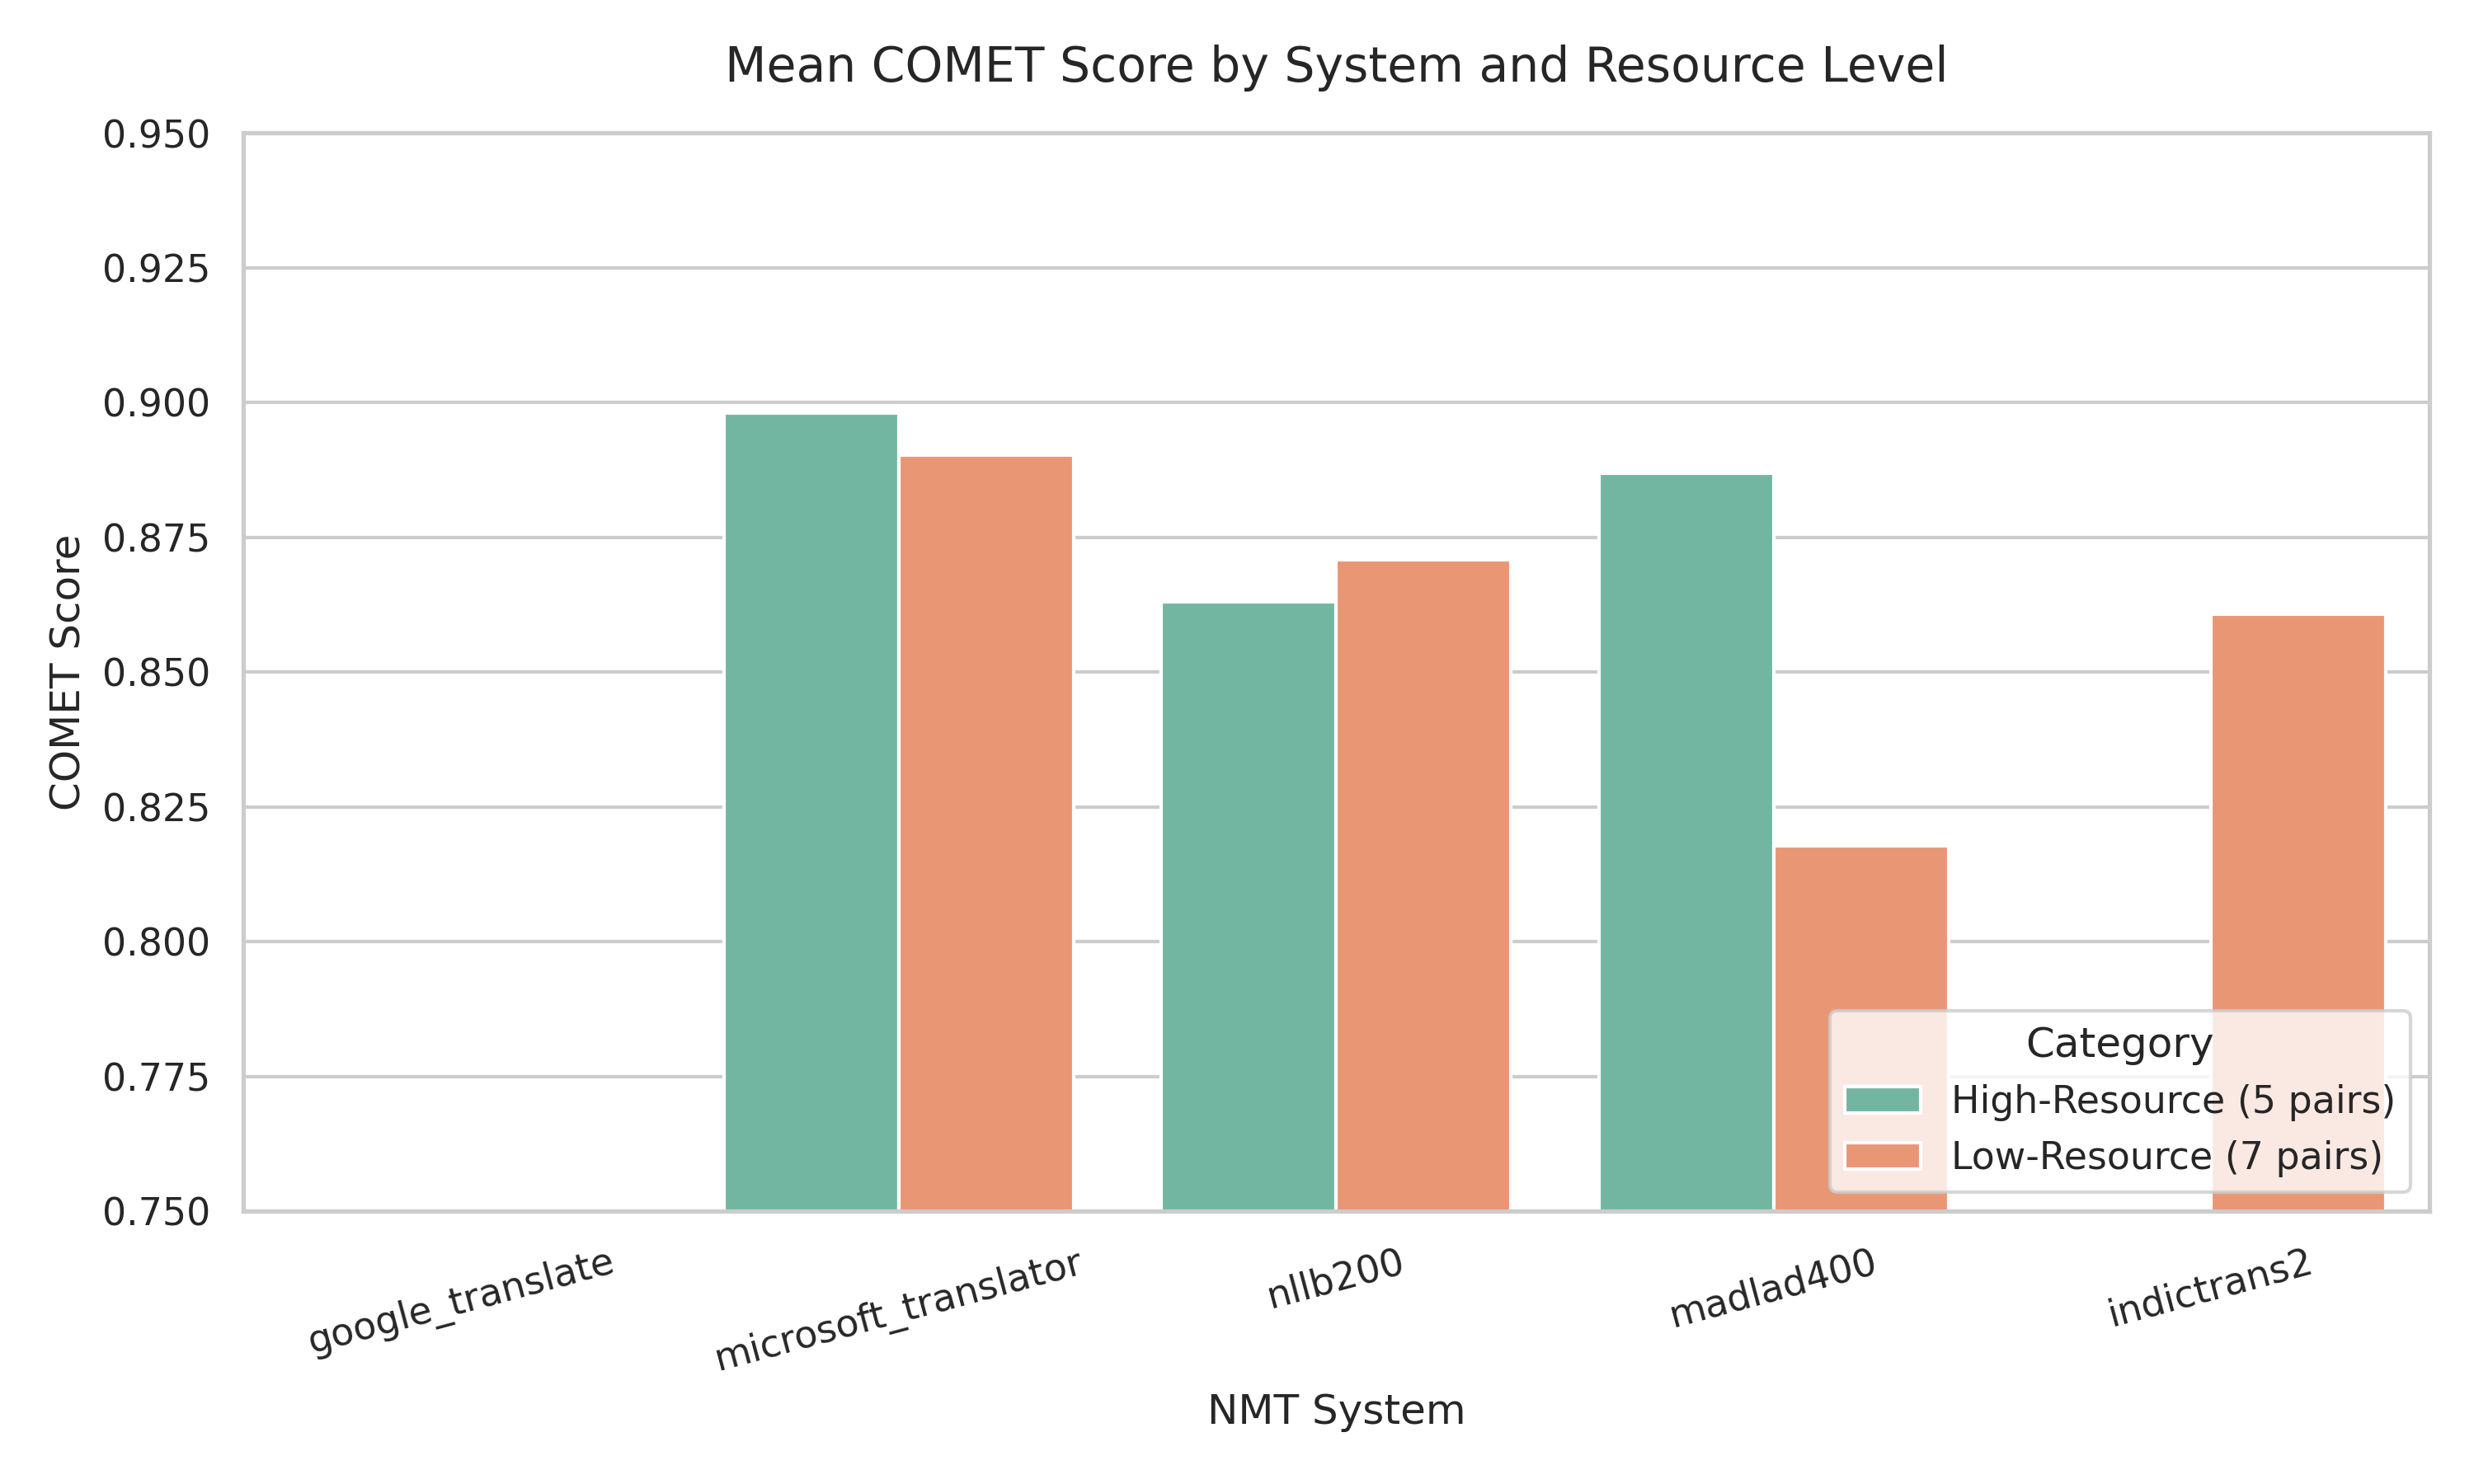
\includegraphics[width=\linewidth]{figures/comet_by_system.png}
\caption{Mean COMET by system for high-resource and low-resource language groups. IndicTrans2 supports only low-resource Indic pairs.}
\label{fig:comet}
\end{figure}

\subsection{Reference-Free Validation (CometKiwi)}

CometKiwi is reference-free: it estimates quality from the source and hypothesis alone, so it can score the Google Translate baseline as a system in its own right and can reveal whether a system that diverges from Google is actually better or worse. Because IndicTrans2 covers only the six Indic languages, Table~\ref{tab:cometkiwi} reports CometKiwi restricted to those six pairs, the only set on which all five systems (including the Google baseline) can be compared fairly.

\begin{table}[h]
\centering
\caption{Reference-free CometKiwi (mean over the six Indic pairs EN-HI, EN-BN, EN-MR, EN-PA, EN-TA, EN-TE), the common subset supported by all five systems.}\label{tab:cometkiwi}
\begin{tabular}{@{}lc@{}}
\toprule
System & CometKiwi \\
\midrule
Google Translate & \textbf{0.803} \\
Microsoft Translator & 0.799 \\
IndicTrans2 & 0.798 \\
NLLB-200 & 0.797 \\
MADLAD-400 & 0.772 \\
\bottomrule
\end{tabular}
\end{table}

On this like-for-like comparison the top four systems are closely bunched (0.797--0.803), with the Google baseline marginally highest, while MADLAD-400 lags slightly behind on this specific domain. Crucially, the reference-free ranking is consistent with the reference-based (COMET) ranking: no system that diverges from Google is revealed to be systematically better than it. This corroborates the benchmarking methodology and confirms that the Indic-specialized system is competitive among open models but does not completely surpass the commercial baseline.

\begin{table}[h]
\centering
\caption{CometKiwi (reference-free) by language, including the Google Translate baseline as an evaluated system. Higher is better. Cross-system comparison is valid only on the six Indic pairs that all five systems cover.}\label{tab:cometkiwi_lang}
\begin{tabular}{@{}lcccccccccccc@{}}
\toprule
System & de & fr & zh & es & ja & hi & ar & bn & mr & pa & ta & te \\
\midrule
Google & 0.789 & 0.781 & 0.778 & 0.791 & 0.811 & 0.805 & 0.761 & 0.817 & 0.783 & 0.807 & 0.804 & 0.800 \\
Microsoft & 0.781 & 0.778 & 0.772 & 0.787 & 0.804 & 0.799 & 0.757 & 0.815 & 0.779 & 0.808 & 0.799 & 0.795 \\
NLLB-200 & 0.777 & 0.777 & 0.741 & 0.780 & 0.793 & 0.806 & 0.753 & 0.815 & 0.780 & 0.800 & 0.792 & 0.786 \\
MADLAD-400 & 0.754 & 0.767 & 0.765 & 0.781 & 0.796 & 0.796 & 0.749 & 0.794 & 0.749 & 0.777 & 0.766 & 0.750 \\
IndicTrans2 & -- & -- & -- & -- & -- & 0.809 & -- & 0.818 & 0.774 & 0.802 & 0.793 & 0.791 \\
\bottomrule
\end{tabular}
\end{table}

Table~\ref{tab:cometkiwi_lang} gives the full per-language reference-free scores. The systems are closely bunched at the language level (most values fall within 0.77--0.81), and no system is uniformly ahead. This reinforces the aggregate finding: reference-free quality does not separate the systems sharply on this UI-string corpus, and the Indic-specialized system does not dominate on the languages it targets.

\subsection{String-Type Analysis}

A distinctive property of software UI strings is the presence of non-linguistic artifacts. Within our corpus, 3.5\% of strings contain variable placeholders (e.g., \texttt{\%1}, \texttt{\%s}) and a smaller fraction contain concatenated camelCase identifiers (e.g., \texttt{rectMeanKineticEnergyVariance}); such tokens must be preserved verbatim, as a corrupted placeholder can break a localized interface at runtime. Because these tokens are meaning-bearing only as literals, they are precisely the cases where surface-level lexical metrics are most informative and where neural metrics, tuned to semantic adequacy, are least sensitive. The short, context-poor nature of UI strings (median two words; 91.9\% of at most three words) further stresses n-gram metrics: BLEU and ROUGE-L are volatile for such strings, since a single differing token can collapse the score, which is consistent with the depressed ROUGE-L values observed for all systems. These observations reinforce our reliance on neural and reference-free metrics for the primary comparison while retaining the lexical metrics for their sensitivity to literal artifact preservation.

To understand the practical impact of translation failures on assistive technology users, we conducted a qualitative error analysis on strings containing critical interface artifacts. When NMT systems fail to preserve these non-linguistic tokens, the resulting errors are not merely cosmetic; they directly degrade software accessibility. For example, in our KDE corpus, software UI strings such as \textit{``globalization''} demonstrated significant vocabulary divergence across models (e.g., Google translating it as \textit{bhumandlikaran} while IndicTrans2 produced \textit{vaishvikaran}). Similarly, technical labels like \textit{``Layer Settings''} highlighted architectural translation differences, where models either utilized phonetic loanwords (\textit{layer settings}) or native technical vocabulary (\textit{parat vinyas}). Preserving these technical nuances without corrupting embedded UI variables remains critical for reliable screen-reader navigation and assistive device performance.

\section{Discussion}

\subsection{System Selection Implications}

Our benchmarking results have direct implications for AI-driven NMT system selection in localization pipelines serving assistive technologies, IoT platforms, and pervasive computing systems. For high-resource European language pairs, commercial systems (Microsoft Translator) and robust multilingual open-source models (MADLAD-400) are expected to closely match or exceed Google Translate quality. For low-resource Indic languages, specialized open-source models (NLLB-200, IndicTrans2) deliver strong alternatives to commercial platforms, suggesting that assistive technology and IoT platforms should implement AI-driven, language-aware routing rather than defaulting to a single NMT provider. This finding is particularly significant for pervasive computing systems deployed in multilingual households, healthcare facilities, and community settings.

Our results refine this expectation. For high-resource pairs the commercial systems align most closely with the Google baseline and score highest on the neural metrics, while open-source models trail slightly. For low-resource Indic pairs, Microsoft Translator is strongest on the reference-based and neural metrics, and, contrary to our initial hypothesis, the Indic-specialized IndicTrans2 does not lead: on the like-for-like reference-free comparison over the six Indic pairs, the systems are closely bunched with IndicTrans2 mid-pack. The practical implication is nuanced: rather than assuming a specialist model is best for underserved languages, pipeline designers should benchmark per language, general-purpose commercial and high-capacity multilingual systems remain competitive, and in some cases preferable, even for low-resource Indic UI content.

\subsection{Metric Reliability for Software UI Content}

Software UI strings, being characteristically short and context-poor, present challenges for evaluation metrics. BLEU, which relies on n-gram overlap, is particularly unreliable for strings of 1 to 3 tokens where a single word difference can cause the score to collapse to zero. Neural metrics (COMET, BERTScore) are expected to provide more reliable assessments by capturing semantic similarity beyond surface-level matching. To empirically quantify the brittleness of lexical overlap metrics on software UI content, we analyzed translation discrepancies across our low-resource language pairs. Filtering for short UI strings (1 to 3 words) where neural adequacy is high ($\text{COMET} \ge 0.85$) but unigram overlap with the Google Translate baseline is completely zero ($\text{intersection} = 0$), we identified 719 verified instances where lexical metrics register a score of zero despite semantic correctness. Qualitative inspection reveals two primary drivers of these false negatives: (1) orthographic and morphological variations (such as alternative punctuation and vowel matras in Indic scripts that share zero exact surface tokens), and (2) valid syntactic paraphrasing, where an open-source model employs a descriptive phrase (e.g., translating \textit{``Uncategorized''} as a descriptive phrase like \textit{``not categorized''}) instead of the baseline compound term. While word-level BLEU collapses to zero in these instances, neural metrics like COMET successfully recognize semantic equivalence.

The CometKiwi reference-free evaluation serves as a critical validation layer, confirming whether reference-based rankings reflect genuine quality differences or are artifacts of the benchmarking methodology. A further consideration is language-specific tokenization. The word-level lexical metrics (METEOR and ROUGE-L) rely on whitespace tokenization and English stemming, and are therefore less reliable for languages that are not space-segmented, notably Chinese and Japanese; for BLEU we mitigate this by applying SacreBLEU's language-specific tokenizers for these languages. This limitation of surface-level lexical metrics reinforces our reliance on neural metrics (COMET, BERTScore, and CometKiwi) as the primary basis for cross-language comparison.

In our results the reference-free CometKiwi rankings are consistent with the reference-based (COMET) rankings on the common language subset, and no system that diverges from the Google baseline is revealed by CometKiwi to be systematically better than it. This agreement validates the benchmarking-against-baseline methodology: the reference-based scores reflect genuine quality differences rather than artifacts of using Google Translate as the reference.

\subsection{Agreement Among Metrics}

To quantify how consistently the eight metrics rank system-language pairs, we computed pairwise Kendall's $\tau$ rank correlations across all evaluated pairs (TER sign-inverted so that higher is better for every metric). The metrics are broadly concordant but far from redundant. Character- and word-overlap metrics correlate most strongly with one another (chrF++ vs. METEOR $\tau=0.70$; chrF++ vs. TER $\tau=0.69$; METEOR vs. TER $\tau=0.77$), confirming that they capture a common surface-similarity signal. The two neural metrics agree moderately (COMET vs. BERTScore $\tau=0.57$), and COMET correlates only weakly-to-moderately with the purely lexical metrics (COMET vs. BLEU $\tau=0.43$; COMET vs. chrF++ $\tau=0.45$), indicating that the neural metrics measure something the surface metrics do not. As Figure~\ref{fig:corr} shows, ROUGE-L is the outlier, correlating weakly with everything ($\tau \leq 0.41$), consistent with its instability on the short, morphologically rich strings in this corpus. These correlations support using neural metrics as the primary basis for comparison while retaining lexical metrics for their sensitivity to literal artifact preservation.

\begin{figure}[h]
\centering
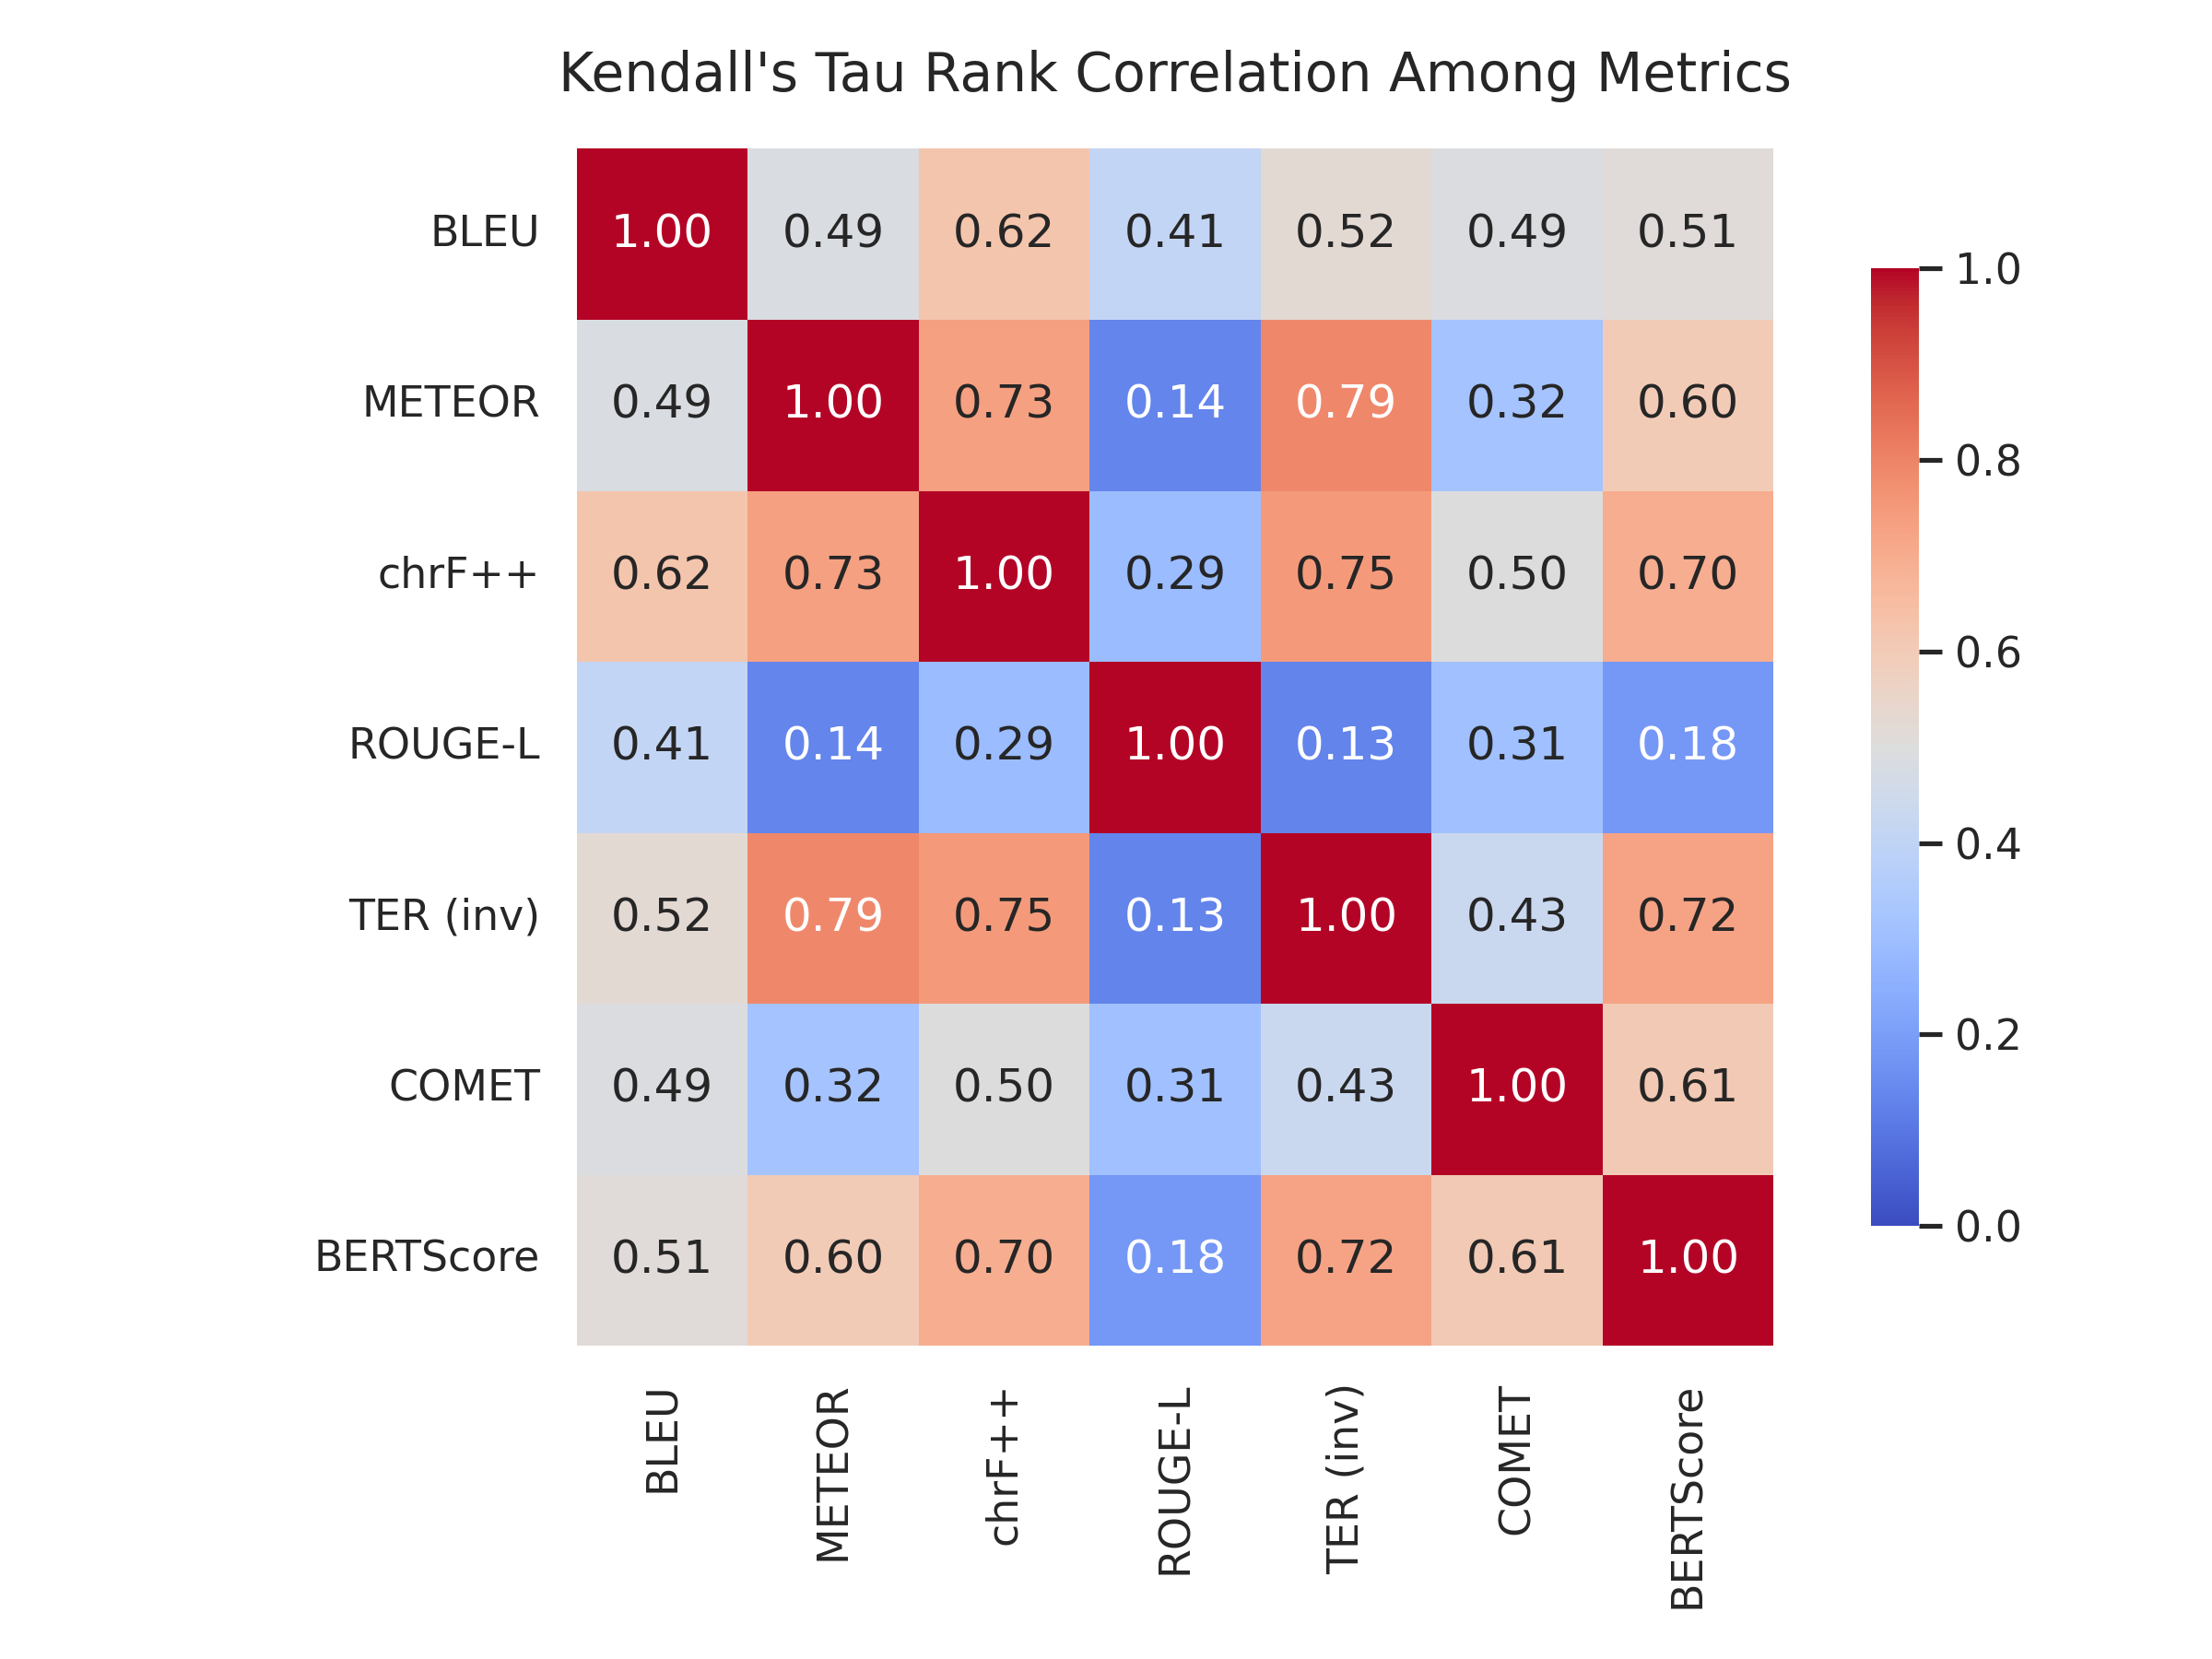
\includegraphics[width=\linewidth]{figures/metric_correlation.png}
\caption{Kendall's $\tau$ rank correlation among the reference-based and neural metrics across all evaluated system-language pairs (TER sign-inverted so higher is better throughout).}
\label{fig:corr}
\end{figure}

\subsection{Implications for Localization Pipeline Design}

Based on our evaluation, we provide the following recommendations for AI-powered localization pipelines in assistive technology, IoT, and pervasive computing environments:

\begin{enumerate}
\item \textbf{Primary quality metric: COMET.} Its high correlation with human judgments and source-aware architecture make it the most reliable metric for quality assessment in automated workflows.
\item \textbf{Secondary metric: chrF++ for morphologically rich languages.} Character-level evaluation is particularly suitable for Indic languages with complex morphology (Hindi, Marathi, Bengali, Tamil, Telugu).
\item \textbf{Reference-free validation: CometKiwi.} Should be deployed alongside reference-based metrics to detect cases where the baseline system (Google Translate) itself produces suboptimal translations.
\item \textbf{Language-aware system routing.} No single NMT system dominates across all language pairs; localization pipelines should route translation requests to the optimal system based on target language resource level.
\end{enumerate}

\subsection{Reproducibility}

To support independent verification, the complete study artifacts are released in the project repository: the fixed set of 10,228 source strings, every system's translation outputs, all evaluation scripts, the computed metric scores, and per-metric result tables. Reproducibility is anchored on pinned software environments rather than a specific machine. The open-source translation systems use deterministic greedy decoding and are pinned via \texttt{requirements-lock.txt} (NLLB-200), \texttt{requirements-madlad400.txt} (MADLAD-400), and \texttt{requirements-indictrans2.txt} (IndicTrans2); the metric computation environment is pinned via \texttt{requirements-metrics.txt}. Because the open models require mutually incompatible library versions, they are documented as separate environments. Model provenance is recorded by Hugging Face commit revision for the open models, and by API access date for the commercial systems, whose server-side models are not version-controllable and whose outputs are therefore retained as frozen snapshots. Byte-level integrity of every released output file is verifiable against published MD5 and SHA-256 checksums. Crucially, all text assets, scripts, and translation outputs strictly utilize Unix \texttt{LF} line endings to ensure cryptographic checksums match across operating systems without \texttt{CRLF} discrepancies. Two of the neural metric models (COMET and CometKiwi) are gated and require access approval, which we note so that reproduction expectations are set accurately.

\subsection{Threats to Validity}

Several limitations bound the interpretation of our results. First, all reference-based metrics measure agreement with the Google Translate baseline rather than against human reference translations; a high score therefore indicates similarity to Google, not certified correctness. We mitigate this with the reference-free CometKiwi metric, whose rankings agree with the reference-based ones, but absolute quality is not established against human judgments. Second, the word-level lexical metrics are unreliable for the non-space-segmented and morphologically rich languages in our set (Chinese, Japanese, and the Indic languages), as discussed in Section~6.2; we therefore weight the neural and reference-free metrics more heavily. Third, the commercial systems (Google, Microsoft) are updated server-side without notice, so their outputs are reproducible only as frozen snapshots at the recorded run dates. Fourth, the evaluation uses a single corpus of software UI strings from one open-source project; results may not transfer to other domains or to longer text. Finally, IndicTrans2 covers only six of the twelve languages, so all cross-system comparisons involving it are restricted to the common Indic subset to avoid the averaging bias that unequal language coverage would otherwise introduce.

\section{Conclusion and Future Work}

This paper presents a comprehensive, AI-driven benchmarking study of NMT systems for multilingual interface localization in assistive technologies, IoT, and pervasive computing environments, using Google Translate as the industry-standard baseline and CometKiwi reference-free quality estimation for independent validation. Our evaluation of four alternative NMT systems, one commercial and three open-source, across twelve language pairs using eight metrics on a fixed set of 10,228 authentic KDE software UI strings provides several key contributions to the artificial intelligence, assistive technology, and pervasive computing communities.

First, we demonstrate that the benchmarking-against-baseline methodology, validated by reference-free quality estimation, produces robust and consistent system rankings for software UI content. Second, we show that NMT system performance hierarchies differ between high-resource and low-resource language pairs, supporting language-aware routing strategies. Third, our analysis of UI string-type-specific challenges reveals that software content requires distinct evaluation approaches compared to standard news or web text.

Future work will focus on: (1) extending the benchmark to LLM-based translation approaches (e.g., GPT-4, Gemini) as AI-driven alternatives to traditional NMT; (2) conducting human evaluation studies with assistive technology end-users to validate system rankings; (3) developing domain-specific NMT fine-tuning for assistive interface content; and (4) evaluating NMT quality in deployed IoT, pervasive computing, and smart home systems across multilingual user populations.

\backmatter

\bmhead{Acknowledgements}

The authors used AI-assisted tools for manuscript preparation, including text drafting and paraphrasing. All content was critically reviewed, verified for accuracy, and edited by the authors, who take full responsibility for the intellectual content and integrity of this work.

\section*{Declarations}

\begin{itemize}
\item \textbf{Funding:} The author(s) received no financial support for the research, authorship, and/or publication of this article.
\item \textbf{Conflict of interest/Competing interests:} The author(s) declared no potential conflicts of interest with respect to the research, authorship, and/or publication of this article.
\item \textbf{Data availability:} The KDE software UI strings originate from the KDE desktop environment, also distributed via the OPUS KDE4 collection at \url{https://opus.nlpl.eu/datasets/KDE4}. The fixed set of 10,228 source strings used in this study, all NMT system outputs, evaluation scripts, pinned dependency versions, run-environment specification, and reproducibility documentation are available in the project repository at \url{https://github.com/Research-SoftwareLocalization/cloud-native-nmt-benchmark}.
\item \textbf{Author contribution:} All authors contributed to the conception and design of the study, the development and evaluation of the benchmarking methodology, and the analysis and interpretation of the results. All authors read, revised, and approved the final manuscript.
\end{itemize}

\begin{thebibliography}{99}

\bibitem{1}
Marcus~A and Gould~EW.
\newblock Globalization, localization, and cross-cultural user-interface design.
\newblock In: Jacko~JA (ed.) \emph{The Human-Computer Interaction Handbook}, 3rd~edn. CRC Press, 2012, pp.~341--366.

\bibitem{2}
Chroust~G.
\newblock Software like a courteous butler: localization under cultural diversity.
\newblock In: \emph{ISSS 2007}.

\bibitem{3}
Banes~D and Draffan~EA.
\newblock A guide to localising assistive technologies.
\newblock In: \emph{ATIA 2013}. Orlando, FL, 2013.

\bibitem{4}
Aqle~A, Al-Masri~A and Nasser~Y.
\newblock Exploring current accessibility challenges in the multilingual web for visually-impaired users.
\newblock In: \emph{Proc 24th Int Conf World Wide Web (WWW 2015 Companion)}. ACM, 2015, pp.~871--872.

\bibitem{5}
Shahin~M, Babar~MA and Zhu~L.
\newblock Continuous integration, delivery, and deployment: a systematic review.
\newblock \emph{IEEE Access} 2017; 5: 3909--3943.

\bibitem{6}
Stahl~D, Martensson~T and Bosch~J.
\newblock Continuous practices and DevOps.
\newblock In: \emph{SEAA 2017}. IEEE, 2017, pp.~440--448.

\bibitem{7}
Sharma~NK, Mate~PD, Pandit~SK, Kar~P, Panda~S and Neti~LBM.
\newblock Cloud-Native Scalable Localization: A Serverless CI/CD Framework for Multilingual Software Delivery.
\newblock In: \emph{2026 IEEE 50th Annual Computers, Software, and Applications Conference (COMPSAC)}. Madrid, Spain: IEEE, 2026, pp.~462--467.

\bibitem{8}
Vaswani~A, Shazeer~N, Parmar~N et~al.
\newblock Attention is all you need.
\newblock \emph{Adv Neural Inf Process Syst} 2017; 30: 5998--6008.

\bibitem{9}
Koneru~S, Huck~M, Exel~M et~al.
\newblock Analyzing challenges in NMT for software localization.
\newblock In: \emph{EACL 2023}, pp.~2442--2454.

\bibitem{10}
Muntes Mulero~V, Paladini Adell~P, Espana Bonet~C et~al.
\newblock Context-aware MT for software localization.
\newblock In: \emph{EAMT 2012}, pp.~77--80.

\bibitem{11}
Hau~E and Aparicio~M.
\newblock Software internationalization and localization in web-based ERP.
\newblock In: \emph{SIGDOC 2008}. ACM, 2008, pp.~175--180.

\bibitem{12}
Giammarresi~S.
\newblock Strategic views on localization project management.
\newblock In: Dunne~KJ and Dunne~ES (eds) \emph{Translation and Localization Project Management}. John Benjamins, 2011, pp.~17--50.

\bibitem{13}
Kab\'{a}t~M.
\newblock Possible translation problems in agile localization of software.
\newblock \emph{Int J Interact Mob Technol} 2023; 17(1).

\bibitem{14}
Lee~S and Yong~HS.
\newblock Distributed agile: project management in a global environment.
\newblock \emph{Empir Softw Eng} 2010; 15: 204--217.

\bibitem{15}
Bola\~{n}os Garc\'{i}a-Escribano~A.
\newblock Cloud technologies in media localisation.
\newblock In: \emph{New Advances in Translation Technology}. Springer, 2024, pp.~55--78.

\bibitem{16}
Gon\c{c}alves~L.
\newblock \emph{Process Improvement for Software Localization} [Master's thesis].
\newblock Helsinki Metropolia University of Applied Sciences, 2011.

\bibitem{17}
Costa-juss\`{a}~MR, Cross~J, \c{C}elebi~O et~al.
\newblock No language left behind: scaling human-centered machine translation.
\newblock \emph{Nature} 2024; 630: 841--846.

\bibitem{18}
Wang~X, Chen~C and Xing~Z.
\newblock Domain-specific machine translation with recurrent neural network for software localization.
\newblock \emph{Empir Softw Eng} 2019; 24(6): 3514--3545.

\bibitem{19}
Smirnov~AV, Teslya~N, Shilov~N et~al.
\newblock Comparative analysis of neural translation models based on Transformers.
\newblock In: \emph{ICEIS (1)}. 2022, pp.~586--593.

\bibitem{20}
Papineni~K, Roukos~S, Ward~T et~al.
\newblock BLEU: a method for automatic evaluation of machine translation.
\newblock In: \emph{ACL 2002}, pp.~311--318.

\bibitem{21}
Banerjee~S and Lavie~A.
\newblock METEOR: an automatic metric for MT evaluation with improved correlation with human judgments.
\newblock In: \emph{Proc ACL Workshop on Intrinsic and Extrinsic Evaluation Measures for MT and/or Summarization}. Ann Arbor, MI, 2005, pp.~65--72.

\bibitem{22}
Popovic~M.
\newblock chrF: character n-gram F-score for automatic MT evaluation.
\newblock In: \emph{WMT 2015}, pp.~392--395.

\bibitem{23}
Lin~CY.
\newblock ROUGE: a package for automatic evaluation of summaries.
\newblock In: \emph{Text Summarization Branches Out}. Barcelona, Spain, 2004, pp.~74--81.

\bibitem{24}
Snover~M, Dorr~B, Schwartz~R et~al.
\newblock A study of translation edit rate with targeted human annotation.
\newblock In: \emph{Proc AMTA 2006}. Cambridge, MA, 2006, pp.~223--231.

\bibitem{25}
Rei~R, Stewart~C, Farinha~AC et~al.
\newblock COMET: a neural framework for MT evaluation.
\newblock In: \emph{EMNLP 2020}, pp.~2685--2702.

\bibitem{26}
Zhang~T, Kishore~V, Wu~F et~al.
\newblock BERTScore: evaluating text generation with BERT.
\newblock In: \emph{ICLR 2020}.

\bibitem{27}
Freitag~M, Rei~R, Mathur~N et~al.
\newblock Results of the WMT22 metrics shared task.
\newblock In: \emph{WMT 2022}, pp.~46--68.

\bibitem{28}
Rei~R, Treviso~M, Yu~N et~al.
\newblock CometKiwi: IST-Unbabel 2022 submission for the quality estimation shared task.
\newblock In: \emph{WMT 2022}, pp.~634--645.

\bibitem{29}
Tiedemann~J.
\newblock Parallel data, tools and interfaces in OPUS.
\newblock In: \emph{Proc 8th Int Conf Lang Resour Eval (LREC 2012)}. Istanbul, Turkey, 2012, pp.~2214--2218.

\bibitem{30}
Gala~J, Chitale~PA, Raghavan~AK et~al.
\newblock IndicTrans2: towards high-quality and accessible machine translation models for all 22 scheduled Indian languages.
\newblock \emph{Trans Mach Learn Res} 2023.

\bibitem{31}
Collins~RW.
\newblock Software localization for Internet software, issues, and methods.
\newblock \emph{IEEE Softw} 2002; 19(2): 74--80.

\bibitem{32}
Esselink~B.
\newblock The evolution of localization.
\newblock \emph{Guide Multiling Comput Technol Localization} 2003; 14(5): 4--7.

\bibitem{33}
Cyr~D and Lew~R.
\newblock Emerging challenges in the software localization industry.
\newblock \emph{Thunderbird Int Bus Rev} 2003; 45(3): 337--358.

\bibitem{34}
Abufardeh~S and Magel~K.
\newblock Software localization: the challenging aspects of Arabic.
\newblock In: \emph{IASTED SE 2008}, pp.~275--279.

\bibitem{35}
Jimenez-Crespo~MA.
\newblock \emph{Localization in Translation}. 2024.

\bibitem{36}
Xia~X, Lo~D, Zhu~F et~al.
\newblock Software internationalization and localization: an industrial experience.
\newblock In: \emph{ICECCS 2013}. IEEE, 2013, pp.~222--231.

\bibitem{37}
Ramler~R and Hoschek~R.
\newblock Automation support for localization testing.
\newblock In: \emph{ICST 2017}. IEEE, 2017, pp.~542--543.

\bibitem{38}
Arjona Reina~L, Robles~G and Gonzalez-Barahona~JM.
\newblock Localization in free software.
\newblock In: \emph{OSS 2013}. Springer, 2013, pp.~153--167.

\bibitem{39}
Kenny~D.
\newblock Human and machine translation.
\newblock In: \emph{Machine Translation for Everyone}. 2022; 18: 23.

\bibitem{40}
Post~M.
\newblock A call for clarity in reporting BLEU scores.
\newblock In: \emph{WMT 2018}, pp.~186--191.

\end{thebibliography}

\end{document}